\documentclass[../../main.tex]{subfiles}

\graphicspath{{\subfix{../../immagini/}}}

\begin{document}
Come illustrato nei paragrafi precedenti i modelli basano la loro efficacia sul valore dei loro parametri (Per questo motivo rientrano nella categoria dei \textit{modelli parametrici}), perciò è necessarrio disporre di tecniche che permettano di ottimizzare, o \textit{apprendere}, il valore di questi parametri. Egual importanza hanno però anche i parametri del modello scelti a priori e non aggiornabili durante l'addestramento, che prendono il nome di \textit{iperparametri}, un semplice esempio di iperparametro è il numero di neuroni in uno strato nascosto di una rete feedforward; la scelta ad esempio di un numero di neuroni molto basso potrebbe portare ad avere un modello non in grado, anche dopo l'addestramento, di rappresentare in modo soddisfacente la funzione obiettivo.

Più nello specifico questo introduce il problema di dover bilalciare tra \textit{bias} e \textit{varianza} di un modello: un bias ridotto indica che il modello è in grado di descrivere bene la distribuzione di dati d'addestramento, viceversa un bias elevato implica un modello non in grado di descrivere neanche il training set, in questo caso parlo di \textit{underfitting}; la varianza indica invece la capacità del modello di generalizzare, quindi di descrivere dati non osservati durante l'addestramento, in caso di alta varianza si parla di \textit{overfitting}.

Scegliere quindi modelli complessi può quindi sfociare in una varianza molto alta, viceversa modelli troppo semplici potrebbero portare ad avere bias ridotto, in questo senso l'obiettivo è di trovare un giusto compromesso tra bias e varianza selezionando iperparametri, o una classe del modello, adeguati.

Non esistono regole che permettono di ricavare il modello migliore in questo senso, spesso si procede quindi analizzando diversi modelli con diverse configurazioni; esistono diverse metriche per quantificare le performance di un modello, quelle utilizzate negli esperimenti vengono descritte nei paragrafi successivi.

\begin{figure}[H]
    \centering
    \begin{subfigure}[t]{0.30\textwidth}
        \centering
        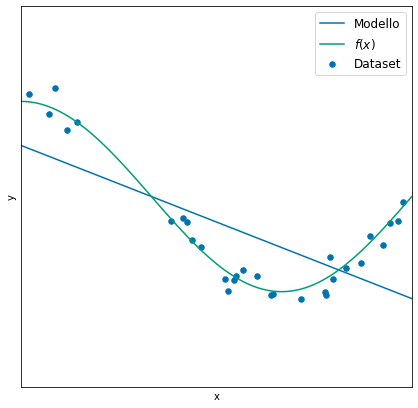
\includegraphics[width=\textwidth]{immagini/4_2/4_2_3/under.png}
        \caption{Esempio di underfitting: il modello dopo l'addestramento non è in grado di descrivere bene neanche i dati d'addestramento.}
    \end{subfigure}
    \begin{subfigure}[t]{0.30\textwidth}
        \centering
        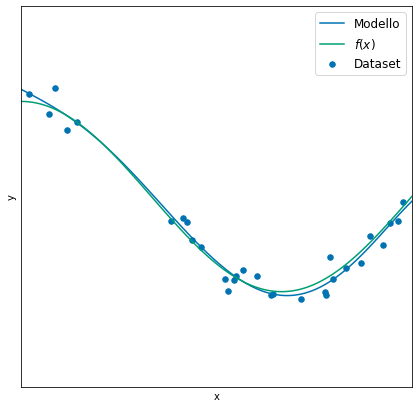
\includegraphics[width=\textwidth]{immagini/4_2/4_2_3/good.png}
        \caption{Esempio di un buon modello, in grado di approssimare correttamente i dati d'addestramento e di fornire una buona generalizzazione.}
    \end{subfigure}
    \begin{subfigure}[t]{0.30\textwidth}
        \centering
        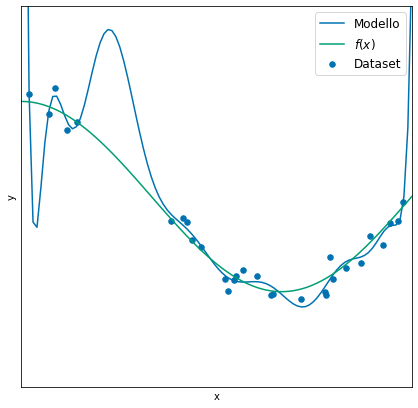
\includegraphics[width=\textwidth]{immagini/4_2/4_2_3/over.png}
        \caption{Esempio di overfitting: il modello dopo l'addestramento è in grado di descrivere correttamente i dati d'addestramento, ma non è in grado di generalizzare.}
    \end{subfigure}
\end{figure}
\end{document}